
\chapter{Estimate Fusion on an Untrusted Cloud}\label{ch:cloud_fusion}

% 
% 8888888b.  8888888b.   .d88888b.  888888b.   
% 888   Y88b 888   Y88b d88P" "Y88b 888  "88b  
% 888    888 888    888 888     888 888  .88P  
% 888   d88P 888   d88P 888     888 8888888K.  
% 8888888P"  8888888P"  888     888 888  "Y88b 
% 888        888 T88b   888     888 888    888 
% 888        888  T88b  Y88b. .d88P 888   d88P 
% 888        888   T88b  "Y88888P"  8888888P"  
%                                              
%                                              
%                                              
% 

\section{Problem Formulation}\label{sec:cloud_fusion:problem}
%Our paper is motivated by a key step in multi-sensor fusion, the requirement of transmitting local sensor state estimates and covariance information over a network for the computation of their fused result. In particular, we consider centralized FCI fusion, where a party responsible for many networked sensors capable of computing their local state estimates, wishes to have their fused state estimate and covariance computed securely on an untrusted cloud. The same party may query the cloud fusion centre for the fused result at any time. To preserve the privacy of local sensor measurements and state estimates, we aim to provide a secure FCI algorithm such that the fusion centre does not learn individual sensor measurements, state estimates, or covariances. This will be achieved by encrypted homomorphic fusion, whereby the untrusted cloud learns only the FCI aggregation weights, which will be shown in section [sec:secfci].

%As we assume the querying party is the owner of all individual sensors, the threat model to be considered is that of network eavesdroppers and a malicious fusion centre, with no possible collusion between sensors and the fusion centre.

%Our proposed filter aims to solve FCI fusion, namely () and (), using only encrypted values from each sensor $i$, and leaking only the weight values $\omega_1,\dots,\omega_n$.

In this work, we consider an arbitrary time-varying process defined by its state $\vec{x}_k \in \mathbb{R}^n$ for all timesteps $k \in \mathbb{N}$. This process is estimated by $m$ individual estimators $i$, $1\leq i\leq m$, each producing a state estimate and an estimate error covariance,
\begin{equation}\label{eqn:ests_and_covs}
    \hat{\vec{x}}_{k,i} \in \mathbb{R}^n \text{ and } \mat{P}_{k,i} \in \mathbb{R}^{n\times n}\,,
\end{equation}
respectively, at every timestep $k$. Our aim at every timestep is for all estimates $\hat{\vec{x}}_{k,i}$ and errors $\mat{P}_{k,i}$, $1\leq i\leq m$, to be sent to a cloud server where a fused estimate and error covariance,
\begin{equation}\label{eqn:fus_ests_and_covs}
    \hat{\vec{x}}_{k,\mathsf{fus}} \in \mathbb{R}^n \text{ and } \mat{P}_{k,\mathsf{fus}} \in \mathbb{R}^{n\times n}\,,
\end{equation}
respectively, are computed and are consistent with the estimates in \eqref{eqn:ests_and_covs}.

Simultaneously, we consider the desired security of the fusion process. The fusing cloud and estimators are treated as \textit{honest-but-curious}, that is, they follow protocols correctly but may use learned information for malicious gain, and a trusted third party exists that can query the cloud at any timestep $k$ to obtain the fusion results in \eqref{eqn:fus_ests_and_covs}. We aim for the cloud, estimators and eavesdroppers to learn no additional information from observed estimates and fusions, \eqref{eqn:ests_and_covs} and \eqref{eqn:fus_ests_and_covs}, respectively, beyond their local estimates. To guarantee this, cryptographic \textit{Indistinguishability under the Chosen Plaintext Attack} (IND-CPA) [katzIntroductionModernCryptography2008] is desired for all transmitted and processed information. This is in line with common security goals in the field and is suitable for homomorphic encryption. The communications of this scenario are summarised graphically in figure [fig:layout].

\begin{figure}[t]
    \centering
    \begin{tikzpicture}
        % Bounding box
        %\draw [gray] (1,-1.5) rectangle (8.5,7);
        % Estimators
        \node at (2.5,6.25) {Estimator $1$};
        \node at (7,6.25) {Estimator $m$};
        \fill [pyplotorange!70] (7,5.5) ellipse (0.5 and 0.5);
        \fill [pyplotorange!70] (2.5,5.5) ellipse (0.5 and 0.5);
        \fill [black] (5,5.5) circle (0.05);
        \fill [black] (4.5,5.5) circle (0.05);
        \fill [black] (4.75,5.5) circle (0.05);
        % Estimates
        \node [right] at (6.25,4.5) {$\hat{\vec{x}}_{k,m},\mat{P}_{k,m}$};
        \node [left] at (3.25,4.5) {$\hat{\vec{x}}_{k,1},\mat{P}_{k,1}$};
        % Fusion
        \node [right] at (5.25,0.5) {$\hat{\vec{x}}_{k,\mathsf{fus}},\mat{P}_{k,\mathsf{fus}}$};
        % Cloud
        \node at (4.75,3.65) {Cloud};
        \fill [pyplotorange!70] (4.75,3) ellipse (0.4 and 0.4);
        \fill [pyplotorange!70] (5.25,2.75) ellipse (0.4 and 0.25);
        \fill [pyplotorange!70] (4.25,2.75) ellipse (0.25 and 0.25);
        \fill [pyplotorange!70] (5.25,3) ellipse (0.25 and 0.25);
        \fill [pyplotorange!70] (4.25,2.5) rectangle (5.25,2.75);
        % Third party
        \node at (4.75,1.25) {Trusted Third party};
        \fill [pyplotblue!70] (5.5,-0.25) -- (4,-0.25) -- (4.75,1);
        % Estimator arrows
        \draw [-latex]  plot coordinates {(3,5)  (4.25,4)};
        \draw [-latex]  plot coordinates {(6.5,5)  (5.25,4)};
        % Third party arrows
        \draw [latex-latex]  plot coordinates {(4.75,2.3)  (4.75,1.65)};
    \end{tikzpicture}
    \label{fig:layout}
\end{figure}

% 
% 8888888888 888     888  .d8888b. 8888888 .d88888b.  888b    888      888      
% 888        888     888 d88P  Y88b  888  d88P" "Y88b 8888b   888      888      
% 888        888     888 Y88b.       888  888     888 88888b  888      888      
% 8888888    888     888  "Y888b.    888  888     888 888Y88b 888      888      
% 888        888     888     "Y88b.  888  888     888 888 Y88b888      888      
% 888        888     888       "888  888  888     888 888  Y88888      888      
% 888        Y88b. .d88P Y88b  d88P  888  Y88b. .d88P 888   Y8888      888      
% 888         "Y88888P"   "Y8888P" 8888888 "Y88888P"  888    Y888      88888888 
%                                                                               
%                                                                               
%                                                                               
% 

\section{Confidential Cloud Fusion Leaking Fusion Weights}

% 
%  ######  ########  ######     ########  ######  #### 
% ##    ## ##       ##    ##    ##       ##    ##  ##  
% ##       ##       ##          ##       ##        ##  
%  ######  ######   ##          ######   ##        ##  
%       ## ##       ##          ##       ##        ##  
% ##    ## ##       ##    ##    ##       ##    ##  ##  
%  ######  ########  ######     ##        ######  #### 
% 

\subsection{Secure Fast Covariance Intersection}

% 
% ..#######...........######..########.##....##
% .##.....##.........##....##.##.......###...##
% ........##.........##.......##.......####..##
% ..#######..#######..######..######...##.##.##
% .##......................##.##.......##..####
% .##................##....##.##.......##...###
% .#########..........######..########.##....##
% 

\subsubsection{Two-sensor Case} \label{sec:secfci}
In this section, we will introduce the Secure FCI (SecFCI) fusion algorithm for the two-sensor case, before extending it to the $n$ sensor case in section [sec:multi\_secfci]. The network model we consider is described in section [subsec:problem\_formulation], where sensors are capable of running local estimators, as well as the PHE and ORE encryption schemes from section [sec:encryption]. Each sensor $i$ computes its state estimate $\mean{\vec{x}}_i$ and covariance matrix $\mP_i$ and sends relevant encrypted information to an untrusted cloud fusion center. The querying party is the key holding party and generates the PHE public key $pk$, secret key $sk$, and ORE symmetric key $k$. $pk$ is made available to all parties in the network, and $k$ is made available to the sensors only, via any standard public-key scheme such as RSA [rivestMethodObtainingDigital1978]. When encrypting with ORE key $k$, individual sensors are limited to using only $L$ or $R$ ORE encryption to reduce local information leakage. Thus, consecutive ORE encryptions from any sensor cannot be used to infer local information directly, and can only be compared to encryptions from sensors using the alternate ORE encryption.

From [eqn:ci\_cov\_estimate], we can see that both CI fusion equations can be computed on PHE encryptions of sensor information vectors and information matrices, given valid unencrypted values for each $\omega_i$. For this reason, we allow the leakage of all weights $\omega_i$. Thus, in the two-sensor case, homomorphic fusion is computed by
\begin{equation}
   \mathcal{E}(\mP^{-1}) = \mathcal{E}(\mP^{-1}_1)^{\omega_1}\mathcal{E}(\mP^{-1}_2)^{(1 -\omega_1)} \label{eqn:paillier_ci_cov}
\end{equation}
and
\begin{equation}
   \mathcal{E}(\mP^{-1}\mean{\vec{x}}) = \mathcal{E}(\mP^{-1}_1\mean{\vec{x}}_1)^{\omega_1}\mathcal{E}(\mP^{-1}_2\mean{\vec{x}}_2)^{(1 - \omega_1)}\enspace, \label{eqn:paillier_ci_estimate}
\end{equation}
where we note that $\omega_2=1-\omega_1$ due to the CI requirement [eqn:ci\_omega\_sum\_bound]. We also note that in [eqn:paillier\_ci\_cov] and [eqn:paillier\_ci\_estimate], each resulting value will have exactly one encoding multiplication factor to remove, and can be decoded exactly by using [eqn:qmn\_mult\_decode].
   
All that remains for computing CI homomorphically, in the two-sensor case, is the calculation of parameter $\omega_1$. For this, we approximate the solution to FCI. Since our encoding scheme in section [subsec:encoding] does not allow division, the exact result of [eqn:fci\_2sen\_omega\_sum\_eq] is approximated. This is accomplished by discretizing $\omega_i$ by step-size $s$, such that $s<1$ and $p=1/s \in \mathbb{Z}$, and approximating [eqn:fci\_2sen\_omega\_sum\_eq] with ORE. An ordered discretization of values $\omega^{(x)}$ is defined by
\begin{equation}
   [\omega^{(1)},\dots,\omega^{(p)}] = [0,s,\dots,1-s,1]\enspace,
\end{equation}
and computed by each sensor $i$. Each $\omega^{(x)}$ is multiplied by $\tr(\mP_i)$ and encrypted with ORE key $k$. Sensor $1$'s list is defined by 
\begin{equation}
   [\mathcal{E}^L_{ORE}(\omega^{(1)}\tr(\mP_1)),\dots,\mathcal{E}^L_{ORE}(\omega^{(p)}\tr(\mP_1))]\enspace, \label{eqn:sen1_ore_list}
\end{equation}
and similarly sensor $2$'s by
\begin{equation}
   [\mathcal{E}^R_{ORE}(\omega^{(1)}\tr(\mP_2)),\dots,\mathcal{E}^R_{ORE}(\omega^{(p)}\tr(\mP_2))]\enspace. \label{eqn:sen2_ore_list}
\end{equation}
Note that Sensor $1$ uses only $L$ ORE while sensor $2$ uses only $R$ ORE, and that both lists are ordered. Lists \eqref{eqn:sen1_ore_list} and \eqref{eqn:sen2_ore_list} are sent alongside PHE encryptions of local information vector and information matrix estimates to the fusion center which uses them to estimate the FCI values of $\omega_1$ and $\omega_2$.

From [eqn:fci\_2sen\_omega\_sum\_eq] we know that $\omega_1$ must satisfy
\begin{equation}
   \omega_1 \tr(\mP_1) = (1-\omega_1)\tr(\mP_2)\enspace. \label{eqn:secfci_2sen_intersect}
\end{equation}
If we reverse \eqref{eqn:sen2_ore_list}, we obtain a list equivalent to one with values $\mathcal{E}^R_{ORE}((1-\omega^{(x)})\tr(\mP_2))$ for each discretization step $x$. When the reversed list is decrypted and plotted over \eqref{eqn:sen1_ore_list} the intersection gives the solution to \eqref{eqn:secfci_2sen_intersect} and therefore, \eqref{eqn:fci_2sen_omega_sum_eq}. However, \eqref{eqn:sen1_ore_list} and reversed \eqref{eqn:sen2_ore_list} consist of $L$ and $R$ ORE encryptions respectively, and the intersection must be approximated by locating consecutive $\omega^{(x)}$ discretizations where the sign of comparisons changes. This can be seen in Fig. \ref{fig:2_sensor_sol}, and can be performed in $O(\log{p})$ ORE comparisons using a binary search.
\begin{figure}[tb]
   \begin{center}
      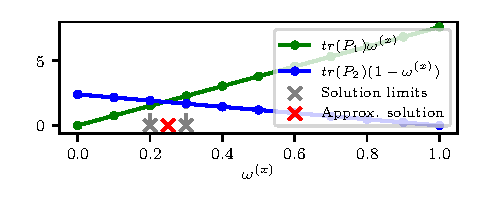
\includegraphics{figures/2_sensors.pdf}
   \end{center}
   \caption{Approximation of $\omega_1$ with discretization step-size $s=0.1$. Only comparisons between line points are used.}
   \label{fig:2_sensor_sol}
\end{figure}
Consecutive $\omega^{(x)}$ and $\omega^{(x+1)}$ for which list comparisons differ can be used to estimate the true intersection, and $\omega_1$, by
\begin{equation}
   \omega_1 \approx 0.5(\omega^{(x)} + \omega^{(x+1)})\enspace. \label{eqn:secfci_2sen_omega}
\end{equation}
In the case a comparison returns equality, the exact value of $\omega^{(x)}$ can be taken to be $\omega_1$.

The fusion center can then use its values for $\omega_1$ and $\omega_2 = 1-\omega_1$ and the received PHE encryptions of local information vectors and information matrices to compute \eqref{eqn:paillier_ci_cov} and \eqref{eqn:paillier_ci_estimate}.

% 
% .##....##..........######..########.##....##
% .###...##.........##....##.##.......###...##
% .####..##.........##.......##.......####..##
% .##.##.##.#######..######..######...##.##.##
% .##..####...............##.##.......##..####
% .##...###.........##....##.##.......##...###
% .##....##..........######..########.##....##
% 

\subsubsection{Multi-sensor Case} \label{sec:multi_secfci}
When computing the SecFCI fusion for $n$ sensors, we solve \eqref{eqn:ci_cov_estimate} homomorphically by computing
\begin{equation}
   \mathcal{E}(\mP^{-1}) = \mathcal{E}(\mP^{-1}_1)^{\omega_1}\cdots\mathcal{E}(\mP^{-1}_n)^{\omega_n} \label{eqn:n_sen_paillier_ci_cov}
\end{equation}
and
\begin{equation}
   \mathcal{E}(\mP^{-1}\mean{\vec{x}}) = \mathcal{E}(\mP^{-1}_1\mean{\vec{x}}_1)^{\omega_1}\cdots\mathcal{E}(\mP^{-1}_n\mean{\vec{x}}_n)^{\omega_n}\enspace. \label{eqn:n_sen_paillier_ci_estimate}
\end{equation}
As with the two-sensor case, encoded results from \eqref{eqn:n_sen_paillier_ci_cov} and \eqref{eqn:n_sen_paillier_ci_estimate} contain exactly one multiplication factor to remove and can be decoded exactly with [eqn:qmn\_mult\_decode]. Again we are just left with the task of computing the plaintext weights $\omega_1,\dots,\omega_n$.

Our approach to the $n$ sensor case is to solve all $n-1$ conditions in \eqref{eqn:fci_eq} using the two-sensor method, and combining partial solutions to compute the final result. When we consider a Euclidean dimension for each $\omega_i$, partial solutions can be considered geometrically as hyperplanes of $n-2$ dimension, over the $n-1$ dimensional solution space given by \eqref{eqn:ci_omega_sum_bound}. 

This can be visualized in the three sensor case, which requires solving partial solutions
\begin{equation}
   \omega_1 \tr(\mP_1) - \omega_2 \tr(\mP_2) = 0,\ \omega_1+\omega_2=1-\omega_3 \label{eqn:3_sensor_partial_sol_1}
\end{equation}
and
\begin{equation}
   \omega_2 \tr(\mP_2) - \omega_3 \tr(\mP_3) = 0,\ \omega_2+\omega_3=1-\omega_1\enspace. \label{eqn:3_sensor_partial_sol_2}
\end{equation}
We can use the two-sensor method from section \ref{sec:secfci} to solve \eqref{eqn:3_sensor_partial_sol_1} exactly when $\omega_3=0$, and know that when $\omega_3=1$, then $\omega_1=\omega_2=0$. These two points are enough to define the two-dimensional partial solution \eqref{eqn:3_sensor_partial_sol_1} which can be seen plotted over the possible solution space in Fig. \ref{fig:3_sensor_partial_sol}. Fig. \ref{fig:3_sensor_partial_sols} shows both partial solutions \eqref{eqn:3_sensor_partial_sol_1} and \eqref{eqn:3_sensor_partial_sol_2} plotted over the solution space.
\begin{figure*}[tb]
   \begin{subfigure}[t]{0.3\textwidth}
      \begin{center}
         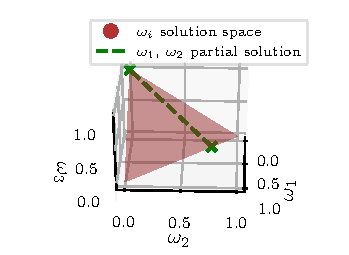
\includegraphics{figures/partial_sol1.pdf}
      \end{center}
      \caption{Partial solution to \eqref{eqn:3_sensor_partial_sol_1}.}
      \label{fig:3_sensor_partial_sol}
   \end{subfigure}
   ~
   \begin{subfigure}[t]{0.3\textwidth}
      \begin{center}
         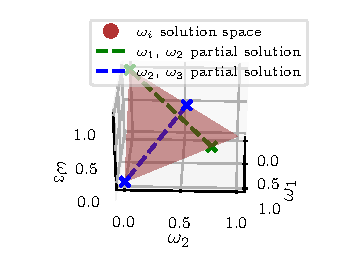
\includegraphics{figures/partial_sols.pdf}
      \end{center}
      \caption{Partial solutions to \eqref{eqn:3_sensor_partial_sol_1} and \eqref{eqn:3_sensor_partial_sol_2}.}
      \label{fig:3_sensor_partial_sols}
   \end{subfigure}
   ~
   \begin{subfigure}[t]{0.3\textwidth}
      \begin{center}
         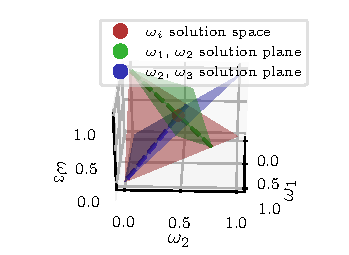
\includegraphics{figures/partial_sol_planes.pdf}
      \end{center}
      \caption{Partial solutions as planes.}
      \label{fig:3sen_planes}
   \end{subfigure}
   \caption{Partial solutions over $\omega_1$, $\omega_2$, and $\omega_3$ solution space.}
   \label{fig:partial_sols_and_planes}
\end{figure*}
The final solution from all partial solutions is computed by finding their intersection. This can be seen in Fig. \ref{fig:3_sensor_partial_sols} as the intersection of the $(\omega_1,\omega_2)$ and $(\omega_2,\omega_3)$ partial solution lines.

To simplify computing the partial solution intersection, we define equivalent planes for each of the partial solutions, perpendicular to the solution space, in the form
\begin{equation}
   a_1\omega_1 + a_2\omega_2 +a_3\omega_3 + a_4 = 0\enspace, \label{eqn:3sen_plane_eq}
\end{equation}
and solve the resulting linear system for finding the intersection of all planes and the solution space. This is given by
\begin{equation}
   \begin{bmatrix}
      a_1^{(1)} & a_2^{(1)} & a_3^{(1)} \\
      a_1^{(2)} & a_2^{(2)} & a_3^{(2)} \\
      1 & 1 & 1
   \end{bmatrix}
   \begin{bmatrix}
      \omega_1 \\
      \omega_2 \\
      \omega_3
   \end{bmatrix}
   =
   \begin{bmatrix}
      a_3^{(1)} \\
      a_4^{(2)} \\
      1
   \end{bmatrix}\enspace, \label{eqn:3sen_plane_sol_eq}
\end{equation}
where $a_i^{(j)}$ denotes parameter $i$ of partial solution $j$, and has been shown visually in Fig. \ref{fig:3sen_planes}.

In the $n$ sensor case, we can similarly solve partial solutions by first using the method from section \ref{sec:secfci} to solve equations with two parameters $\omega_k$ and $\omega_{k+1}$ when letting all $\omega_i=0,\ i\neq k,k+1$. For each equation we can then compute remaining partial solution points at $\omega_i=1,\ i\neq k,k+1$ with $\omega_j=0,\ j\neq i$. Perpendicular hyperplanes can then be similarly defined in the form 
\begin{equation}
   a_1\omega_1 + \dots +a_n\omega_n + a_{n+1} = 0\enspace. \label{eqn:nsen_plane_eq}
\end{equation}
Due to their inherent orthogonality, and that all meaningful covariance traces are strictly positive, the $n-1$ partial solution hyperplanes are guaranteed to intersect at exactly one point. The hyperplane intersection results in the linear system 
\begin{equation}
   \begingroup
   \setlength\arraycolsep{2pt}
   \begin{bmatrix}
      a_1^{(1)} & a_2^{(1)} & \cdots & a_{n}^{(1)} \\
      \vdots & \vdots & \ddots & \vdots \\
      a_1^{(n-1)} & a_2^{(n-1)} & \cdots & a_{n}^{(n-1)} \\
      1 & 1 & \cdots & 1
   \end{bmatrix}
   \begin{bmatrix}
      \omega_1 \\
      \vdots \\
      \omega_{n-1} \\
      \omega_{n}
   \end{bmatrix}
   \!=\!
   \begin{bmatrix}
      a_{n+1}^{(1)} \\
      \vdots \\
      a_{n+1}^{(n-1)} \\
      1
   \end{bmatrix}\enspace, \label{eqn:hyperplane_sol_eq}
   \endgroup
\end{equation}
and gives the solution to the SecFCI $\omega_i$ weights.

As all $O(n\log{p})$ ORE comparisons are done between sequential sensors $i$ and $i+1$, $L$ and $R$ ORE encryptions can be used to the same effect as for the two-sensor case. The ORE ordered list sent from each sensor $i$ is given by
\begin{equation}
   \begin{aligned} \label{eqn:sensor_lists}
      &[\mathcal{E}^L_{ORE}(\omega^{(1)}\tr(\mP_i)),\dots,\mathcal{E}^L_{ORE}(\omega^{(p)}\tr(\mP_i))],\,i\text{ odd} \\
      &[\mathcal{E}^R_{ORE}(\omega^{(1)}\tr(\mP_i)),\dots,\mathcal{E}^R_{ORE}(\omega^{(p)}\tr(\mP_i))],\,i\text{ even}.
   \end{aligned}
\end{equation}
When combining \eqref{eqn:sensor_lists} with PHE encryptions of local information vectors and information matrices, SecFCI can be computed entirely homomorphically by \eqref{eqn:n_sen_paillier_ci_cov} and \eqref{eqn:n_sen_paillier_ci_estimate}.

Briefly considering the security of our scheme, we note that any leaked information from ORE lists \eqref{eqn:sensor_lists}, as described in [chenettePracticalOrderRevealingEncryption2016], can be considered a subset of knowing the estimated fusion weights $\omega_1,\dots,\omega_n$, which specify relative sizes of sensor covariance traces, and we already consider public. Thus only IND-CPA and IND-OCPA (after accounting for leakage through public weights) encryptions are made available to the fusion centre.

% 
%  ######   #######  ##     ## ########  
% ##    ## ##     ## ###   ### ##     ## 
% ##       ##     ## #### #### ##     ## 
% ##       ##     ## ## ### ## ########  
% ##       ##     ## ##     ## ##        
% ##    ## ##     ## ##     ## ##        
%  ######   #######  ##     ## ##        
% 

\subsection{Computational Complexity} \label{subsec:complexity}
Given the state estimates and estimate errors at each sensor, we wish to show the computational complexity of the SecFCI algorithm for the $n$ sensor case. We will assume that both Lewi ORE and Paillier PHE schemes use the same length security parameter (and equivalently key size), such that $\lambda_{Lewi} = \lambda_{Paillier} = \log{N}$, where $\lambda_{s}$ represents encryption scheme $s$'s security parameter, and $N$ the Paillier modulus and encryptable integer limit. We also note the distinction between floating-point or small integer operations, which are typically treated as having $O(1)$ runtime, and large integer operations whose complexities are dependent on bit length. While architectures exist for speeding up encryption operations [gueronIntelAdvancedEncryption2010], we consider software implementations and treat large integer operations in terms of bit operations explicitly.

From [paillierPublicKeyCryptosystemsBased1999,lewiOrderRevealingEncryptionNew2016], and the assumptions made above, we have summarized the operation complexities of the two schemes in Table \ref{tab:complex_ops}.
\begin{table}[tb]
   \centering
   \caption{Computation complexity of encryption operations.}
   \label{tab:complex_ops}
   \begin{tabular}{ |c|c| }
      \hline
      \textbf{Operation} & \textbf{Complexity} \\ 
      \hline
      Paillier enc. & $O(\log^3{N})$ \\ 
      Paillier dec. & $O(\log^3{N})$ \\ 
      Paillier add. & $O(\log^2{N})$ \\ 
      Paillier scalar mult. & $O(\log^3{N})$ \\ 
      Lewi $L$ enc. & $O(\log^2{N})$ \\ 
      Lewi $R$ enc. & $O(\log^2{N})$ \\ 
      Lewi comp. & $O(\log^2{N})$ \\ 
      \hline
   \end{tabular}
\end{table}
In contrast to some current FHE schemes, these operations are of a much lower complexity than [vandijkFullyHomomorphicEncryption2010a], which has complexity $O(\lambda^{10})$ for integer operations, and [stehleFasterFullyHomomorphic2010], which computes single bit operations in $O(\lambda^{3.5})$ adding significant overhead for integer arithmetic.

Finally, applying the operations from Table \ref{tab:complex_ops} to the SecFCI algorithm, we summarize the total complexity of SecFCI at the sensors and the fusion centre in Table \ref{tab:complex}, with the unencrypted complexities of FCI shown for reference. 
\begin{table}[tb]
   \centering
   \caption{Computation complexity at sensors and fusion centre.}
   \label{tab:complex}
   \begin{tabular}{ |c|c|c| }
      \hline
       & \textbf{FCI} & \textbf{SecFCI} \\ 
      \hline
      Sensors & $O(1)$ & $O\left(p\log^2{N} + \log^3{N}\right)$ \\ 
      Fusion & $O(n^3)$ & $O\left(n\log{p}\log^2{N} + n\log^3{N} + n^3\right)$ \\ 
      \hline
   \end{tabular}
\end{table}

% 
%  ######  ########  ######  
% ##    ## ##       ##    ## 
% ##       ##       ##       
%  ######  ######   ##       
%       ## ##       ##       
% ##    ## ##       ##    ## 
%  ######  ########  ######  
% 

\subsection{Security Analysis}

% 
%  ######  #### ##     ## 
% ##    ##  ##  ###   ### 
% ##        ##  #### #### 
%  ######   ##  ## ### ## 
%       ##  ##  ##     ## 
% ##    ##  ##  ##     ## 
%  ######  #### ##     ## 
% 

\subsection{Simulation} \label{sec:results}
We have implemented a simulation to demonstrate the accuracy of SecFCI approximating FCI. Three sensors independently measure a constant-speed linear process and simultaneously run a Kalman filter on their measurements. Estimates are sent both encrypted and unencrypted to a fusion centre that computes the SecFCI and FCI fusions on the received data respectively. Encrypted estimates are comprised of PHE encryptions of the information vector and information matrix, $\mathcal{E}(\mP^{-1}_i\mean{\vec{x}}_i)$ and $\mathcal{E}(\mP^{-1}_i)$, in addition to the ORE list given by \eqref{eqn:sensor_lists} with discretization step $s=0.1$. Unencrypted estimates consist of the state estimate $\mean{\vec{x}}_i$ and covariance $\mP_i$. The trajectory and fused estimates are shown in Fig. \ref{fig:fci_secfci_traj}.
\begin{figure}[tb]
   \begin{center}
      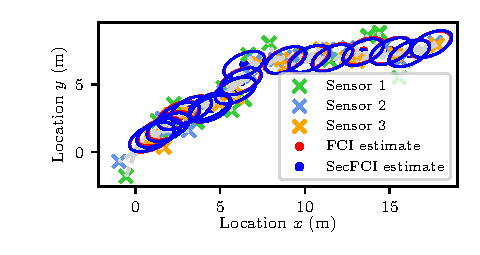
\includegraphics{figures/fci_secfci_cmp.pdf}
   \end{center}
   \caption{Tracking simulation comparing SecFCI and FCI.}
   \label{fig:fci_secfci_traj}
\end{figure}

To derive an upper bound on the accuracy difference between SecFCI and FCI, we note the two factors which introduce inconsistency between the two methods: the encoding method from section \ref{subsec:complexity}, and the difference in fusion weights. Due to the possibility of choosing sufficiently large integer and fractional bit lengths $i$ and $f$, we will only consider the error caused by the difference in weights. We will treat this error as the distance between respective weight vectors
\begin{equation}
   \begin{aligned}
      &\vec{\omega}_{SecFCI} = (\omega_{1,SecFCI},\dots,\omega_{n,SecFCI}) \\
      &\vec{\omega}_{FCI} = (\omega_{1,FCI},\dots,\omega_{n,FCI})\enspace,
   \end{aligned}
\end{equation}
where $\omega_{i,s}$ denotes weight $\omega_i$ from algorithm $s$. From section \ref{sec:secfci} we see that the largest difference $|\omega_{i,FCI} - \omega_{i,SecFCI}|$ is strictly bounded by $s/2$. As shown in section \ref{sec:multi_secfci}, when more sensors are involved, a tighter bound on this difference is dependent on the value of $\vec{\omega}_{i,FCI}$, but will remain strictly bounded by $s/2$. Therefore, we can give a strict upper bound on the distance between weight vectors as
\begin{equation}
   |\vec{\omega}_{FCI} - \vec{\omega}_{SecFCI}| < 0.5\sqrt{ns^2}\enspace. \label{eqn:accuracy_error_bound}
\end{equation}

Finally, components of $\omega_{i,SecFCI}$, $\omega_{i,FCI}$ and the errors $|\vec{\omega}_{FCI} - \vec{\omega}_{SecFCI}|$, have been plotted over time in Fig. \ref{fig:fci_secfci_omegas}, and show the computed error bound when $n=3$ and $s=0.1$.
\begin{figure}[tb]
   \begin{center}
      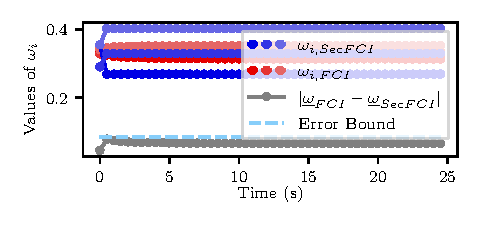
\includegraphics{figures/omegas_cmp.pdf}
   \end{center}
   \caption{$\vec{\omega}_{SecFCI}$ and $\vec{\omega}_{FCI}$ components.}
   \label{fig:fci_secfci_omegas}
\end{figure}

% 
% 8888888888 888     888  .d8888b. 8888888 .d88888b.  888b    888      888b    888 888      
% 888        888     888 d88P  Y88b  888  d88P" "Y88b 8888b   888      8888b   888 888      
% 888        888     888 Y88b.       888  888     888 88888b  888      88888b  888 888      
% 8888888    888     888  "Y888b.    888  888     888 888Y88b 888      888Y88b 888 888      
% 888        888     888     "Y88b.  888  888     888 888 Y88b888      888 Y88b888 888      
% 888        888     888       "888  888  888     888 888  Y88888      888  Y88888 888      
% 888        Y88b. .d88P Y88b  d88P  888  Y88b. .d88P 888   Y8888      888   Y8888 888      
% 888         "Y88888P"   "Y8888P" 8888888 "Y88888P"  888    Y888      888    Y888 88888888 
%                                                                                           
%                                                                                           
%                                                                                           
% 

\section{Confidential Cloud Fusion Without Leaking Fusion Weights}

With the problem and preliminaries introduced, we can now present our encrypted FCI method that leaks no estimator information to the fusing cloud. The core idea behind the method is to postpone the evaluation of operations that cannot be performed homomorphically until partial results are queried and decrypted by the key-holding third party. The remaining operations can then be evaluated on unencrypted inputs to produce the correct results.

First, we note that the FCI fusion equations [eqn:ci\_cov\_fusion] and [eqn:ci\_est\_fusion] can be rearranged and substituted with weights [eqn:fci\_weights] to obtain the equations
\begin{equation}\label{eqn:fci_cov_rearrange}
    \mat{P}_{k,\mathsf{fus}} = \left(\left(\sum_{i=1}^m \frac{1}{\tr(\mat{P}_{k,i})}\right)^{-1}\sum_{i=1}^m \frac{1}{\tr(\mat{P}_{k,i})}\mat{P}_{k,i}^{-1}\right)^{-1}
\end{equation}
and
\begin{equation}\label{eqn:fci_est_rearrange}
    \hat{\vec{x}}_{k,\mathsf{fus}} = \mat{P}_{k,\mathsf{fus}}\left(\sum_{i=1}^m \frac{1}{\tr(\mat{P}_{k,i})}\right)^{-1}\sum_{i=1}^m\frac{1}{\tr(\mat{P}_{k,i})}\mat{P}_{k,i}^{-1}\hat{\vec{x}}_{k,i}\,.
\end{equation}
In this form, innermost summations  
\begin{equation}
    \begin{split}
        \sum_{i=1}^m \frac{1}{\tr(\mat{P}_{k,i})}\,,\ \sum_{i=1}^m &\frac{1}{\tr(\mat{P}_{k,i})}\mat{P}_{k,i}^{-1}\text{ and }\\ 
        &\qquad\sum_{i=1}^m\frac{1}{\tr(\mat{P}_{k,i})}\mat{P}_{k,i}^{-1}\hat{\vec{x}}_{k,i}
    \end{split}
\end{equation}
combine information from individual estimators $i$ and are computable homomorphically given suitable encryptions. Encryptions of these sums can then be decrypted by the key-holding third party, before remaining inversions and multiplications in \eqref{eqn:fci_cov_rearrange} and \eqref{eqn:fci_est_rearrange} can be computed to obtain the final results. To depict this process, pseudocode for the encryption at estimators, fusion at the cloud and decryption by the third party are provided in algorithms~\ref{alg:est_enc}, \ref{alg:cloud_fus} and \ref{alg:fus_query}, respectively.
\begin{algorithm}[htbp]
\caption{Estimator Encryption}\label{alg:est_enc}
\begin{algorithmic}[1]
    \setstretch{1.35}
    \Procedure{Estimate}{$i$, $k$, $\mathsf{pk}$, $\phi$}
    \State Estimate $\hat{\vec{x}}_{k,i}$ locally
    \State Estimate $\mat{P}_{k,i}$ locally
    \LineComment{Public key is encoding and encryption modulus}
    \State $N \gets \mathsf{pk}$
    \LineComment{Encode scaling, covariance and estimate components}
    \State $\tilde{s}_{k,i} \gets \mathsf{E}_{N,\phi}\left(\frac{1}{\tr(\mat{P}_{k,i})}\right)$
    \State $\tilde{\mat{C}}_{k,i} \gets \mathsf{E}_{N,\phi}\left(\frac{1}{\tr(\mat{P}_{k,i})}\mat{P}_{k,i}^{-1}\right)$
    \State $\tilde{\vec{e}}_{k,i} \gets \mathsf{E}_{N,\phi}\left(\frac{1}{\tr(\mat{P}_{k,i})}\mat{P}_{k,i}^{-1}\hat{\vec{x}}_{k,i}\right)$
    \LineComment{Encrypt scaling, covariance and estimate components}
    \State $s_{k,i} \gets \mathcal{E}_{\mathsf{pk}}\left(\tilde{s}_{k,i}\right)$
    \State $\mat{C}_{k,i} \gets \mathcal{E}_{\mathsf{pk}}\left(\tilde{\mat{C}}_{k,i}\right)$
    \State $\vec{e}_{k,i} \gets \mathcal{E}_{\mathsf{pk}}\left(\tilde{\vec{e}}_{k,i}\right)$
    \State Send $s_{k,i}$, $\mat{C}_{k,i}$ and $\vec{e}_{k,i}$ to fusing cloud
    \EndProcedure
\end{algorithmic}
\end{algorithm}
\begin{algorithm}[htbp]
\caption{Cloud Fusion}\label{alg:cloud_fus}
\begin{algorithmic}[1]
    \setstretch{1.35}
    \Procedure{Fuse}{$k$, $\mathsf{pk}$}
    \State Receive $s_{k,i}$, $\mat{C}_{k,i}$ and $\vec{e}_{k,i}$ for all $1\leq i \leq m$
    \State $N \gets \mathsf{pk}$
    \State $s_k \gets \prod_{i=1}^{m} s_{k,i} \pmod{N^2}$
    \State $\mat{C}_k \gets \otimes_{i=1}^{m} \mat{C}_{k,i} \pmod{N^2}$
    \State $\vec{e}_k \gets \otimes_{i=1}^{m} \vec{e}_{k,i} \pmod{N^2}$
    \State Store $s_k$, $\mat{C}_k$ and $\vec{e}_k$ in case of query
    \EndProcedure
\end{algorithmic}
\end{algorithm}
\begin{algorithm}[htbp]
\caption{Fusion Query}\label{alg:fus_query}
\begin{algorithmic}[1]
    \setstretch{1.35}
    \Procedure{GetResult}{$k$, $\mathsf{pk}$, $\mathsf{sk}$, $\phi$}
    \State Query and receive $s_k$, $\mat{C}_k$ and $\vec{e}_k$ from fusing cloud
    \State $N \gets \mathsf{pk}$
    \LineComment Decrypt
    \State $\tilde{s}_k \gets \mathcal{D}_{\mathsf{sk}}\left(s_k\right)$
    \State $\tilde{\mat{C}}_k \gets \mathcal{D}_{\mathsf{sk}}\left(\mat{C}_k\right)$
    \State $\tilde{\vec{e}}_k \gets \mathcal{D}_{\mathsf{sk}}\left(\vec{e}_k\right)$
    \LineComment Decode
    \State $\bar{s}_k \gets \mathsf{E}^{-1}_{N,\phi}\left(\tilde{s}_k\right)$
    \State $\bar{\mat{C}}_k \gets \mathsf{E}^{-1}_{N,\phi}\left(\tilde{\mat{C}}_k\right)$
    \State $\bar{\vec{e}}_k \gets \mathsf{E}^{-1}_{N,\phi}\left(\tilde{\vec{e}}_k\right)$
    \LineComment Compute Fusion
    \State $\mat{P}_{k,\mathsf{fus}} \gets \left(\bar{s}_k^{-1} \cdot \bar{\mat{C}}_k\right)^{-1}$
    \State $\hat{\vec{x}}_{k,\mathsf{fus}} \gets \mat{P}_{k,\mathsf{fus}} \cdot \bar{s}_k^{-1} \cdot \bar{\vec{e}}_k$
    \State \Return $\hat{\vec{x}}_{k,\mathsf{fus}}$, $\mat{P}_{k,\mathsf{fus}}$
    \EndProcedure
\end{algorithmic}
\end{algorithm}

\begin{remark}\label{rem:seq_extension}
    Along with allowing the summations to be performed homomorphically on the cloud, we note that this form of the FCI also allows the cloud's partial fusion operations to be evaluated sequentially. This can be seen in algorithm~\ref{alg:cloud_fus}, where individual components $s_{k,i}$, $\mat{C}_{k,i}$ and $\vec{e}_{k,i}$ from each estimator can continue to be aggregated as additional estimators send their estimate information. This, in turn, supports the dynamic joining and leaving of estimators in the network without affecting the cloud or the operations of a trusted third party. The security implications of such an extension are discussed further in section~\ref{subsec:security}.
\end{remark}

% 
%  ######   #######  ##     ## ########  
% ##    ## ##     ## ###   ### ##     ## 
% ##       ##     ## #### #### ##     ## 
% ##       ##     ## ## ### ## ########  
% ##       ##     ## ##     ## ##        
% ##    ## ##     ## ##     ## ##        
%  ######   #######  ##     ## ##        
% 

\subsection{Computational Complexity}\label{sec:complexity}
The method described provides a level of security when relying on an untrusted cloud for fusing estimates. However, the added reliance on an encryption scheme and the additional computations at the third party intuitively increase the computational complexity of the algorithm and the required capabilities of participating parties. Here, we present the complexity of operations during fusion, required by each party at every timestep $k$. We assume encoding and decoding operations have complexity $O(1)$ (due to their comparative insignificance when compared to associated encryption and decryption operations) and use \cite{paillierPublicKeyCryptosystemsBased1999} to obtain the encryption complexities of the Paillier encryption scheme in table \ref{tab:enc_cmplx}, with security parameter $\lambda = \log{N}$.
\begin{table}[tb]
    \centering
    \caption{Computation complexity of encryption operations.}
    \label{tab:enc_cmplx}
    \begin{tabular}{|c|c|}
       \hline
       \textbf{Operation} & \textbf{Complexity} \\ 
       \hline
       Encryption & $O(\log^3{N})$ \\ 
       Decryption & $O(\log^3{N})$ \\ 
       Addition & $O(\log^2{N})$ \\ 
       Scalar mult. & $O(\log^3{N})$ \\ 
       \hline
    \end{tabular}
 \end{table}
In table \ref{tab:fus_cmplx}, we compare the complexities of the unencrypted FCI algorithm and the method presented in this work.
\begin{table}[tb]
    \centering
    \caption{Computation complexity at parties during fusion.}
    \label{tab:fus_cmplx}
    \begin{tabular}{ |c|c|c| }
       \hline
        & \textbf{FCI} & \textbf{Our Method} \\ 
       \hline
       Estimator & $O(1)$ & $O\left(n^2\log^3{N}\right)$ \\ 
       Fusion & $O(mn^3)$ & $O\left(mn^2\log^2{N}\right)$ \\ 
       Third party & $O(1)$ & $O\left(n^2\log^3{N} + n^3\right)$ \\ 
       \hline
    \end{tabular}
 \end{table}
It can be seen that the burden of computation is greatly increased at the estimators and the third party, in particular when dimension $n$ is large and when a long encryption key $N$ is used. Naturally, an application of the proposed method would need to consider these requirements in terms of computation time and required hardware.

% 
%  ######  ########  ######  
% ##    ## ##       ##    ## 
% ##       ##       ##       
%  ######  ######   ##       
%       ## ##       ##       
% ##    ## ##       ##    ## 
%  ######  ########  ######  
% 

\subsection{Security Analysis}\label{subsec:security}
The provable security of the presented method is relatively straightforward. Our aim for IND-CPA security of all information received by the cloud, sent by the estimators or observable by eavesdroppers is achieved by the homomorphic Paillier encryption scheme. Since all transmitted information is encrypted and the cloud, estimators and eavesdroppers do not hold the secret key $\mathsf{sk}$, IND-CPA is met at all parties.

We note, however, an implicit assumption made when encrypting multidimensional data element-wise. While individual elements are indistinguishable, element-wise encryption does not encrypt the estimate's dimension $n$, which remains implicitly public. While existing methods allow the complete homomorphic encryption of vectors [alexandruPrivateWeightedSum2020], they are left for future work and considered beyond the scope of this work. Instead, we acknowledge the implicit leakage of $n$ and note that, while this may leak information about the fusion's use case, state estimates remain hidden. Additionally, intuitive extensions to the scheme, such as the dynamic joining and leaving of estimators in remark \ref{rem:seq_extension}, may introduce further implicit leakages that must be considered if security is analysed. In this example, the periodic estimation may leak to the cloud when estimators are within an estimation range or context, and a solution may be sending dummy measurements with $s_{k,i}=\mathcal{E}_{\mathsf{pk}}(\mathsf{E}_{N,\phi}(0))$ when estimator $i$ is out of range. This extension is presented only as an example of when care needs to be taken to maintain desired security goals, but in general, extensions and solutions are task-dependent and not a focus of this work.


% 
%  ######  #### ##     ## 
% ##    ##  ##  ###   ### 
% ##        ##  #### #### 
%  ######   ##  ## ### ## 
%       ##  ##  ##     ## 
% ##    ##  ##  ##     ## 
%  ######  #### ##     ## 
% 
\subsection{Simulation}\label{sec:simulation}
Fusion estimates and error covariances from the proposed encrypted FCI method differ from unencrypted FCI only when quantisation errors are large or summation overflows occur. As stated in section [subsec:encoding], when the Paillier modulus $N$ is large, these errors can often be considered negligible. In this section, we demonstrate this similarity in performance between the encrypted and unencrypted FCI fusion algorithms with a simulation. Code was written in the Python programming language, using the $\mathsf{phe}$ Paillier encryption scheme library [PythonPaillier2013] and a $512$ bit length key (bit length of $N$). The simulation implements a linear constant velocity model,
\begin{equation}\label{eqn:sim_sys_model}
    \vec{x}_k =
    \begin{bmatrix}
        1 & 0.5 & 0 & 0\\
        0 & 1 & 0 & 0\\
        0 & 0 & 1 & 0.5\\
        0 & 0 & 0 & 0
    \end{bmatrix}
    \cdot \vec{x}_{k-1} + \vec{w}_k\,,
\end{equation}
with noise term $\vec{w}_k \sim \mathcal{N}(\vec{0}, \mat{Q})$ and
\begin{equation}
    \mat{Q} = 10^{-3} \cdot
    \begin{bmatrix}
        0.42 & 1.25 & 0 & 0\\
        1.25 & 5 & 0 & 0\\
        0 & 0 & 0.42 & 1.25\\
        0 & 0 & 1.25 & 5
    \end{bmatrix}\,.
\end{equation}
At each timestep $k$, the system state $\vec{x}_k$ is estimated by $m=4$ estimators, $1\leq i \leq 4$, using a standard linear Kalman filter (KF) [haugBayesianEstimationTracking2012] and producing estimates and error covariances $\hat{\vec{x}}_{k,i}$ and $\mat{P}_{k,i}$, respectively. The measurements used by the KF, $\vec{z}_{k,i}$, follow the measurement models
\begin{equation}
    \vec{z}_{k,i} = 
    \begin{bmatrix}
        1 & 0 & 0 & 0\\
        0 & 0 & 1 & 0
    \end{bmatrix}
    \cdot \vec{x}_k + \vec{v}_{k,i}\,,
\end{equation}
with noise terms $\vec{v}_{k,i} \sim \mathcal{N}(\vec{0}, \mat{R}_i)$ and covariances sampled indepedently, resulting in
\begin{equation}
    \begin{split}
        &\mat{R}_1 = 
        \begin{bmatrix}
            4.77 & -0.15\\
            -0.15 & 4.94
        \end{bmatrix}\,,\ 
        \mat{R}_2 = 
        \begin{bmatrix}
            2.99 & -0.55\\
            -0.55 & 4.44
        \end{bmatrix}\,,\\
        &\mat{R}_3 = 
        \begin{bmatrix}
            2.06 & 0.68\\
            0.68 & 1.96
        \end{bmatrix}\text{ and }
        \mat{R}_4 = 
        \begin{bmatrix}
            1.17 & 0.80\\
            0.80 & 0.64
        \end{bmatrix}\,.
    \end{split}
\end{equation}
The fusion results of $1000$ simulation runs are shown in figure \ref{fig:sim_error_plot}. 
\begin{figure}[htbp]
    \centering
    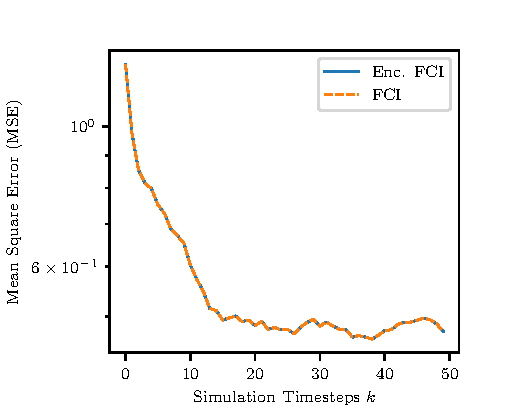
\includegraphics{figures/sim_error_plot.pdf}
    \caption{Average RMSE of encrypted and unencrypted FCI fusion over $1000$ simulations.}
    \label{fig:sim_error_plot}
\end{figure}
From the figure, we can see the expected similarity in performance between the encrypted and unencrypted FCI methods. Additionally, we note that the current recommended key length for the Paillier encryption scheme is $2048$ bits [barkerRecommendationPairWiseKey2019], easily supporting a modulus $N$ and fractional precision $\phi$ that guarantee similar performance.

% 
%  .d8888b.   .d88888b.  888b    888  .d8888b.  
% d88P  Y88b d88P" "Y88b 8888b   888 d88P  Y88b 
% 888    888 888     888 88888b  888 888    888 
% 888        888     888 888Y88b 888 888        
% 888        888     888 888 Y88b888 888        
% 888    888 888     888 888  Y88888 888    888 
% Y88b  d88P Y88b. .d88P 888   Y8888 Y88b  d88P 
%  "Y8888P"   "Y88888P"  888    Y888  "Y8888P"  
%                                               
%                                               
%                                               
% 

\section{Conclusions on Confidential Estimate Fusion}

%FCI is a commonly used, and efficiently computable, approximation to the CI optimization problem that requires the sharing of local sensor estimates to compute their fusion. We propose a secure approximation to FCI, SecFCI, to compute the fused estimate homomorphically. The novel encrypted fusion approach may find uses in various security-critical applications or over untrusted networks subject to eavesdroppers and malicious participants. Possible future work includes run-time comparisons with FHE implementations, giving a computational bound for its practicality, and quantification of fusion weight leakages via formal security proofs.

%In this work, we have presented a method for computing encrypted Fast Covariance Intersection homomorphically on an untrusted cloud and discussed its security guarantees. The method ensures no estimator information leakage at the cloud, eavesdroppers or other estimators and an accompanying simulation demonstrates its minimal effect on estimation performance when compared to the unencrypted algorithm. Applications include a variety of distributed fusion tasks when external fusing computations are required such as weather forecasting and vehicle localisation. Future work on the topic aims to extend the method to include multivariable encryption, hiding the dimension variable $n$, and generalising to decentralised environments where individual fusing parties are untrusted.